\chapter{Feature Extraction}
    In this chapter we discuss the different approaches for extracting features from the music. The basis for all our methods are the mel spectrograms, which we extract from songs of the free music archive (FMA) dataset~\cite{FMA}, giving us a decent selection of 8 different genres.

\section{Mel Spectrograms}
    In sound processing, it is difficult to work with the raw signal of any music track.
    Usually the signal is sampled 22050 to 44100 times per second and therefore yields a lot of data points to be processed. 
    Feeding this signal directly to a neural network is inconvenient and single data points don't give a lot of information.
    A way to counter this problem is the short-time Fourier transform. 
    It applies the Fourier transformation on a window of the signal, returning the individual frequencies present at that time frame. 
    Then the window is moved by a given step size, usually smaller than the frame to include some overlap, and the transformation is repeated.
    This results in a spectrogram with information about the magnitude of the individual frequencies and their change over time.\\
    \begin{figure}[!b]
        \centering
        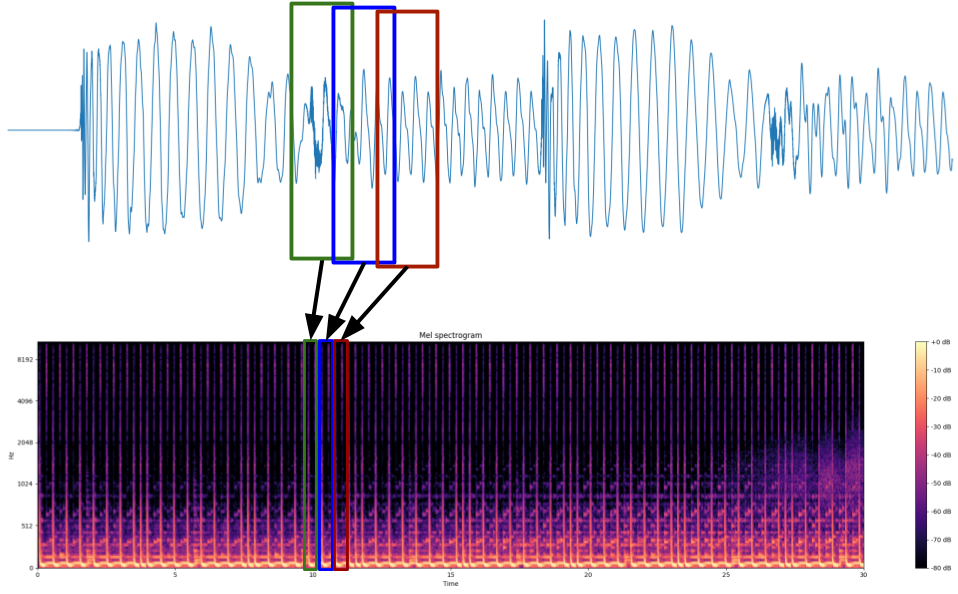
\includegraphics[width=0.8\textwidth]{images/sigToMels.png}
        \caption{The mel spectrogram represents the power of the different frequencies in a frame as they change over time. The powers are mapped to a decibel scale.}
        \label{mel}
    \end{figure}
    \indent Mel spectrograms are an extension of the short-time Fourier transform, which map the magnitudes of the frequencies to a logarithmic power scale, to better approximate the human perception of sound.
    For our experiments we sampled the songs with 22050Hz and chose a frame size of $2^{11}=2048$ samples for the transformation.
    This corresponds to a window of about 100ms, as bursts of frequencies, which are shorter than this time frame, are perceived less loud by the human ear~\cite{Acoustics}.\\
    To be able to produce 60 fps videos from the music, we chose the step size to be $\lfloor \frac{22050}{60} \rfloor = 367$, also introducing a reasonable amount of overlap, and 128 buckets for the frequencies as the resolution of the spectrum.
    As a last step, we mapped the powers of the mel spectrogram to a decibel scale from -80 to 0, to directly display the sound level of a frequency.\\ 
    \indent Figure~\ref{mel} shows a plot of a mel spectrogram obtained from a 30 second sound snippet of an electronic music track. 
    The recurrent bass line is clearly visible in the visualization, already yielding more visible information about the song than the raw signal.
    These mel spectrograms are the basis for every of our approaches.

\section{Autoencoder}
    For our second feature method, we trained an autoencoder to reduce the dimensionality of the mel spectrograms.
    \begin{figure}[!t]
        \centering
        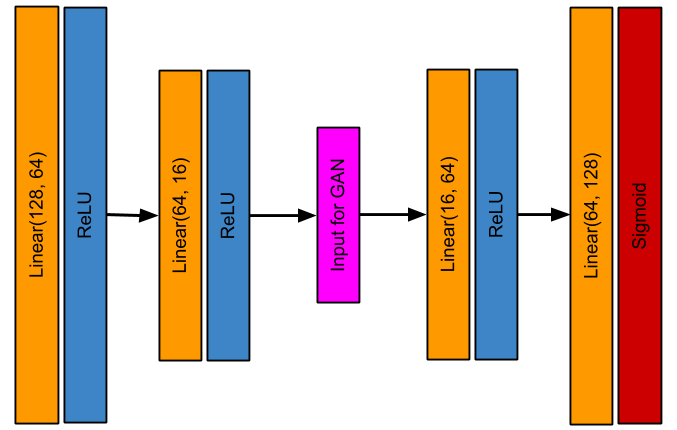
\includegraphics[width=0.75\textwidth]{images/autoencoder}    
        \caption{Architecture of the autoencoder}
        \label{autoencoder}
    \end{figure}
    Figure~\ref{autoencoder} shows the architecture of the neural network, which we used to encode the vectors. In the first step, we half the dimensionality to 64 dimensions, followed by a rectified linear unit (ReLU).
    The next layer reduces the dimensionality down to the encoded size of 16 dimensions, followed by another ReLU. 
    The resulting vectors then serve as potential source of input for a GAN.\\
    The decoding side of the network is symmetric to the encoding side, but ends with the sigmoid function. As the sigmoid function scales the values between 0 and 1, we have to divide the vectors of the mel spectrogram by -80 (they range from -80 to 0) before we put them into the autoencoder, scaling them between 0 and 1 as well. In order to restore the original mel spectrogram, we therefore have to multiply the decoded vectors with -80.\\
    As our loss function, we used the MSELoss (mean squared L2 norm) to measure the error between each element of the decoded vector and the original target vector. 
    We trained this setup for 400 epochs.
    Figure~\ref{reconstructed} shows a reconstruction of the mel spectrogram from Figure~\ref{mel}, after been passed through the fully trained autoencoder.
    The overall structure of the original spectrogram is clearly maintained, indicating that the autoencoder loses little information in the 16 dimensions of the encoded layer, but the reconstruction is a bit blurry, smoothes out information and has slightly different magnitudes than the original. This result is sufficient for our purpose.

    \begin{figure}
        \centering
        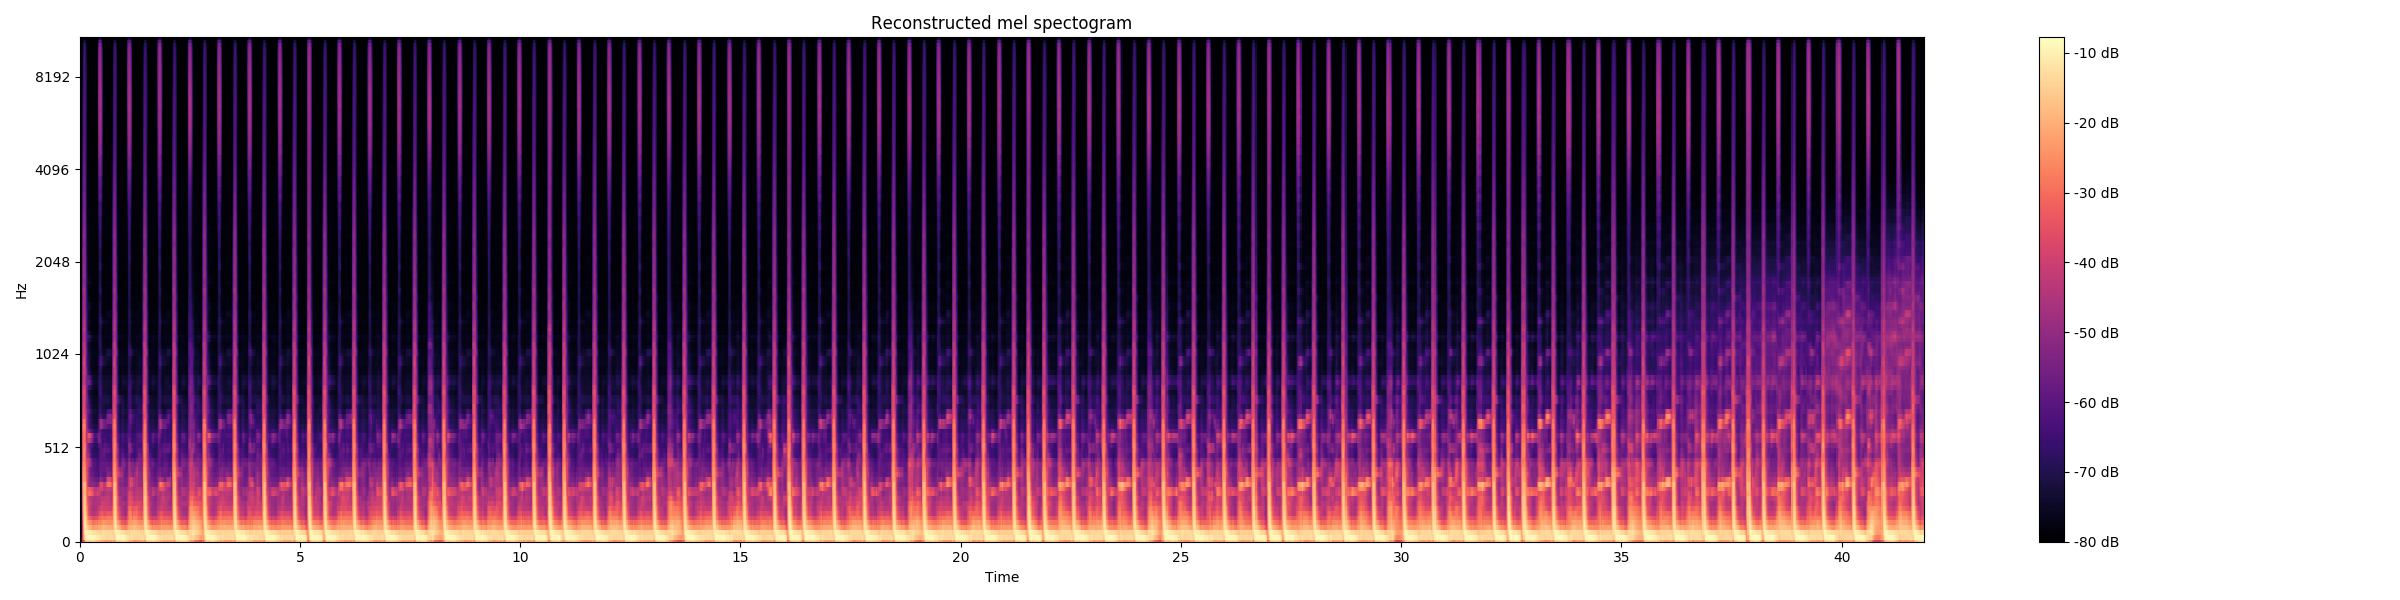
\includegraphics[width=\textwidth, trim=0 0 220 0, clip]{images/recon_spec}
        \caption{Reconstructed mel spectrogram after being encoded and decoded again by our fully trained autoencoder.}
        \label{reconstructed}
    \end{figure}
    
\section{Convolutional Recurrent Neural Network}

    \TODO{CRNN stuff!}
    \begin{figure}[b]
        \centering
        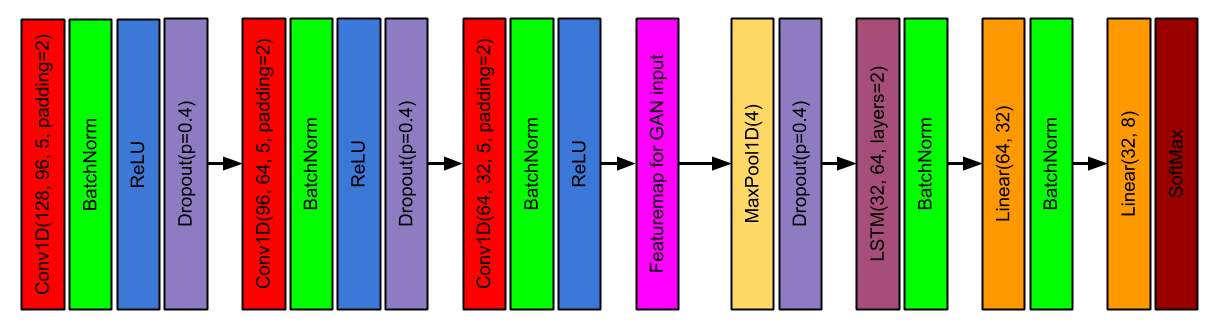
\includegraphics[width=\textwidth]{images/CRNNmodel}
        \caption{Architecture of the convolutional recurrent neural network.}
        \label{CRNN}
    \end{figure}